\section{Design} \label{design}

After the literature study, the design phase started. First, the MuiCSer framework is briefly explained as this was used throughout development of the prototype. Next, the dashboard solution was proposed following the literature study. Hereafter, personas and scenarios hint at the functionality and usage of this dashboard. Last, the components of the system, together with design choices, are described and visualized with paper-mockups.

    \subsection{MuiCSer} \label{2_muicser}
    % description of process
    This section describes the MuiCSer framework, made for user-centered software engineering processes in a multidisciplinary context \cite{muicser}, which was used to create the dashboard prototype. This framework focuses on optimizing the user experience during the entire software engineering cycle to ensure that the needs of the end user are fulfilled. By combining user-centered design methodologies and software engineering principles, the user experience of the final product can be improved substantially.

        \subsubsection{Process}
        
        \begin{figure}[!t]
            \centering
            
\includegraphics[width=0.8\textwidth]{chapters/3_design/muicser}
            \caption{MuiCSer process}\label{fig:muicser}
        \end{figure}

        The MuiCSer process is summarized in figure \ref{fig:muicser}. After each phase, the result is evaluated, verified and validated to ensure that the required functionality is present. In turn, the received feedback can be used to reiterate over the previous phase. On the figure, this is denoted with the light arrows, while the dark one represents the overall process direction. What follows is a brief description of each phase:

        \paragraph{New or legacy system} At the start of the MuiCSer process an existing system in need of improvement is either evaluated or a new one will be designed. This requires an analysis of the tasks and needs of the user, as well as the objects and resources required to perform these tasks. Personas and scenarios are the resulting artifacts of this phase. First, personas describe the personalities of the potential end users including hobbies, skills and the environment they surround themselves in \cite{persona_scenario}. Its goal is to uncover behavior patterns which can be of use when designing a user interface. Second, scenarios tell stories describing the use of a fictitious system from the point of view of a persona \cite{persona_scenario}. It tries to sketch the usage of the system for which a design must be made. These artifacts are found in section \ref{3_personas_scenarios}.

        \paragraph{Structured interaction analysis} During this phase, the results of the analysis are used to create task models. These models specify concrete tasks and goals which can be dissected into specific actions or steps the user has to take. These artifacts lay the foundation for designing a user interface which supports these tasks and goals. Task models were not created. However, each component of the dashboard tries to support certain tasks. These are described in section \ref{design_modules}.

        \paragraph{Low fidelity prototyping} When the actions have been specified using the task models, low fidelity prototypes are designed. Paper sketches and mockups are such examples and are ideal for visualizing the layout of the user interface. Without spending too much time and resources, presenting such prototypes can yield valuable feedback from the end-user or customer. However, there is no interaction present. Typically multiple versions of these prototypes are created until the customer is satisfied, after which high fidelity prototypes can be developed. For each component description in section \ref{design_modules}, low fidelity prototypes are presented. If some of these are too similar, then they are found in appendix \ref{app_low_fidelity}.

        \paragraph{High fidelity prototyping} Creating high fidelity prototypes requires a lot more effort compared to low fidelity prototypes, as they offer functionality closely resembling the final product. However, the feedback will be much more valuable as not only design, but also functionality is tested. Section \ref{implementation} describes the process of creating the prototype featured in this thesis. Choice of frameworks and design changes compared to the low fidelity prototypes are also mentioned in this section.

        \paragraph{Final user interface} When the latest iteration of the high fidelity prototype satisfies all user requirements, the final user interface can be created. It would be beneficial to reuse the code from the prototype in order to save time and resources. As a final step, the task models are checked against the interface to check if all required functionality is present. In this case, the high fidelity prototype is the final product of this thesis. As such, this phase was not reached.

    \subsection{Proposal}
    
    The proposal features four core concepts which will be combined to form one cohesive solution: a dashboard, telemonitoring of chronic diseases, customization, and integration. As mentioned in the introduction, multiple applications and integrating them pose several difficulties: data is spread and stored multiple times. Interaction between these applications is initially not present and integration with existing systems requires a significant amount of work from the IT staff of the institution. As more applications are added, this becomes increasingly difficult. To remedy this problem, each application becomes a module which can be plugged into the dashboard system.

    A module-based approach towards the dashboard allows easy customization and integration. Each module will serve its own purpose by showing data for one particular health parameter. As mentioned in section \ref{2_telemonitoring}, parameters such as heart rate and blood pressure are often measured to monitor multiple chronic diseases. Integration is handled by the fact that each module is independent and does not require other modules to work properly. This also helps with customization as a clinician can choose which modules are relevant for the patient in question.

    The modules that will be developed are for use in chronic disease monitoring. However, modules can be developed for purposes more fit for in-patient care. Examples are real-time monitoring, documenting diagnoses, and viewing of lab results. Which modules will be implemented and what each one of them tries to achieve is described in section \ref{design_modules}. The implementation section will provide more insight on how this independence is achieved and how future modules can be easily integrated.

    This combination allows the clinician to customize the dashboard according to the needs of each patient, facilitating effective care. Data is found rapidly, albeit summarized or detailed, and not hidden away behind multiple screens. Developers should be able to create modules that will fit into the dashboard, negating the use of multiple applications. The following section describes how the system will work and how the users interact with it.

    \subsection{Personas \& scenarios} \label{3_personas_scenarios}

    Based on the proposal mentioned in the previous section, personas and scenarios have been created to get a better understanding of its users and how the system will work. Each of these tries to highlight the problems the users face and how the new system tries to solve them.

        % highlights customization and dashboard
        \subsubsection{Jake}

        \paragraph{Persona} Jake is a 25-year-old male who currently works as a nurse at the hospital in his city. He has been working there for four years and lives alone in his apartment. Still being a young adult, Jake grew up with technology. As a result, he experiences no difficulties when using new software on his computer or smartphone. His hobbies include music, playing the guitar, and video gaming.

        Currently, the workflow at the hospital is dated. A new health information system was introduced to summarize and gather all medical data in a singular space. Because this is an all-in-one system, a lot of features that Jake does not need still clutter the screen. Navigating the system is difficult and customization is not present. Jake wishes to only see the features he uses most while hiding the features he does not need.
        
        \paragraph{Scenario} Jake starts his first day using the new system by reading the manual that is accompanied with it. He starts the application and for each patient he is presented with a list of modules that can be added to the dashboard. These modules can help with the following: cardiovascular disease, respiratory disease, diabetes, and others.

        After selecting a few modules, Jake is presented with a dashboard. The dashboard contains all the wanted functionality of the system, where each ``block'' represents a module that was added. Jake moves a few blocks around until he is satisfied with the layout. He noticed a module he does not need anymore and promptly deletes it by selecting the option on the module. After a while, Jake got transferred to another department and wants to add a new module to support his new workflow. He opens the module list and selects the he wants, which is then added to the dashboard.

        By examining the new module Jake quickly notices that on the dashboard a summary is given. But when Jake clicks on the enlarge button, the module expands to fill a larger area where detailed information is shown. Jake feels he is in control of the system and that it will improve his productivity.\\

        \noindent This scenario highlights the benefits of customization. Hiding unwanted components, while adding the useful ones allow for a clear dashboard to be displayed. The user is in control and is able to quickly view data of importance. It is still possible to view detailed data.
        
        % highlights customization
        \subsubsection{Dan}

        \paragraph{Persona} Dan is a general practitioner since he graduated from university. He is on the job for 21 years and he is the preferred doctor in his town. Throughout the years Dan has used a multitude of systems and he always tries new ones to improve his workflow. Because he has been a general practitioner for such a long time, he has 500 patients that visit him at least twice a year. Some patients, especially the elderly, visit as much as once a month.

        Most of Dan's patients visit for illnesses such as fever and a cold. To diagnose these illnesses no data is necessarily needed, just a description of the patient's symptoms will suffice most of the time. If Dan performs such a diagnosis, he promptly adds it to the information system and to the electronic health record of the patient.

        However, if a patient visits that has a lot of problems regarding his blood pressure, then Dan has to perform a more complex diagnosis using historical data. In the current system that Dan uses, it is very difficult to search for this data. But what bugs Dan the most is that he has to do it every time this patient visits.

        \paragraph{Scenario} Because of Dan's ongoing curiosity, he tries a new health information system which allows customization for each specific patient. Because the diagnoses of most patients can be very different from time to time, Dan creates a default module group which is displayed for each patient, unless that patient has a specific module configuration. The default module group includes past diagnoses, known allergies, patient information (blood type, last weight, height\ldots), and a current medication list.

        The first patient of the day describes what sounds like a fever. Dan confirms this and hands the patient a prescription. The diagnosis is added to the `past diagnoses' module and the prescribed medication to the `current medication list' module. Dan did not need other health data to perform the diagnosis. Therefore, Dan does not change the configuration of this patient.

        The next patient, an elderly woman, came for her second visit of this month. Dan knows from the past that it will probably be a heart related problem. Dan searches for a `heart' module and adds it to the configuration of the elderly woman. Now both the default module group and a heart rate module are present, which is unnecessary according to Dan. He removes some modules of the default module group. Now, the next time the elderly woman visits, that configuration will be automatically loaded.

        One specific patient had broken his arm three times in less than a year. When the patient came for a routine visit, Dan immediately added a module to easily view x-ray photos and view them in a timeline.\\

        \noindent Again, the benefits of system customization for each patient are obvious. Initially, it will take some time to configure each dashboard for all the patients, but the system will try to make this process quick to complete. Once the configuration is done, the time spent during a consultation will decrease.
        
        % highlights telemonitoring
        \subsubsection{Emily}

        \paragraph{Persona} Just like Dan, Emily has been a successful general practitioner for quite some time. However, she has different needs of an EHRS. Between each patient visit, there is a period of time in which Emily does not know what happens to patients regarding certain parameters. For example, if a person has to regularly measure his heart rate and blood pressure because of cardiovascular disease, it is imperative that the doctor is made aware of these values. If Emily sees that these values are not looking well, she can contact the patient to come in for a checkup.

        If a patient has sleep issues, Emily wishes to not see detailed measurement values, but regular descriptions of the night’s sleep. This includes the hours of sleep, amount of wake-ups, subjective feeling of tiredness. Currently, Emily has no way of regularly receiving this information without having the patient visit.
        
        \paragraph{Scenario} Emily recently received notice of a new platform that includes telemonitoring support. Several mobile applications are developed that can send data using an API to the platform, which in turn processes the values and can notify Emily of any anomalies. It includes customization for certain parameters in which Emily can individually assign thresholds for each patient.

        A patient who recently had a cardiac arrest is continuing rehabilitation at home. However, the patient has chest pains and pays Emily a visit. She tells the patient to regularly measure his blood pressure and heart rate, and to take note of these values in a mobile application. This application also allows taking general notes, such as feeling pain or having caught a cold. After they have scheduled the next visit, the patient is sent home.
        
        As the next few weeks pass by, Emily is notified that this patient has crossed a threshold regarding his blood pressure. Immediately Emily checks the measured data and sees a graph of all measured values. This dataset delivers insight into the history of the patient and Emily sees that there is currently no need to panic. She decides to not take action and configures a weekly reminder to keep monitoring the blood pressure.
        
        The next week, Emily receives a notification that the patient has made a note. It reads that he experienced chest pains. Again, Emily takes a look at the blood pressure data and sees a worsening trend leading to hypertension. Emily decides to call the patient to schedule an early visit. The system helped Emily to intervene as soon as the situation seemed to worsen while avoiding having the patient visit too early which in turn saves Emily time.
        
        Another patient has sleep issues. Emily encourages the patient to use a sleep monitor, which is a wristband. This device is connected to a smartphone which communicates the quantitative data to the new platform. The application on the smartphone allows the patient to take note of qualitative data such as a general description of the night or what food he ate. One night the patient slept only three hours and took note that he went out and drank a lot of alcohol. This could explain for example the bad sleeping rhythm for the next few days. Emily wishes to keep track of this patient on a weekly basis and configures the platform to notify her.\\

        \noindent Here, the effects of telemonitoring are highlighted. By generating reports and alerts, the caregiver can intervene when necessary. Combine this with the aforementioned dashboard platform, greater efficiency of care can be accomplished.

        % highlights integration
        \subsubsection{Anna}

        \paragraph{Persona} Anna is a software engineer working at the local hospital. From the early 2000's, she was responsible for the integration of health software systems. As such, she has experienced the continuous change associated with health software. Each unit of the hospital uses different software, while they all share a general system to view patient records. The interaction between these applications is one of Anna's responsibilities.

        As time goes on, new software and medical instruments that improve workflow are purchased. Sometimes these replace old systems, otherwise they are added to work alongside them. Both are becoming increasingly difficult to do, as the codebase of the EHRS grows. When an older system gets replaced, Anna has to weed through the code and delete little pieces, hoping other parts wont break. It is a frustrating task as often band-aid solutions are applied.

        \paragraph{Scenario} A new EHRS was installed that should improve integration of other applications. Anna skims through the documentation and starts the transition process. She quickly notices that for each device or application she needs to create a back end data structure and a module that represents it in the EHRS. The new EHRS is designed that these modules can serve as complete standalone applications or be part of a larger set of modules.

        After the initial transition period, everything is put into place. Not soon after, new bedside monitors with accompanying software were purchased. These replace the old bedside monitors and consequently, the software. Thanks to the new EHRS, Anna deletes the old module without much hassle. Also, she reworked the back end data structure to work with the readings from the new device. The data of the old device is ported to the new data structure, so no data is lost. Anna designed the new module to be similar in appearance and functionality. After implementing the module, the staff barely notices any change and workflow resumes with minor disruption.\\

        \noindent This persona and scenario highlight the importance of integration. Significant time and effort can be saved if this process is simplified. Also, maintenance is easier due to looser coupling of the modules.

    \subsection{Modules} \label{design_modules}
    
    As mentioned in the proposal, the dashboard will feature a module-based design. This section describes the modules that will be available in the prototype. For each module, the reasons behind the design choices are given, as well as a low-fidelity paper mockup. Keep in mind that all modules are primarily chosen to aid with chronic disease management, due to the customization possibilities. Each module has a design which is in line with the principles mentioned in section \ref{2_dashboards}. For each module we ask the following questions:
    \begin{itemize}
        \item What functionality does the module offer?
        \item What data will it represent?
        \item How do we show as much data as possible at a glance?
        \item How are summaries generated?
        \item How are the detailed values shown?
    \end{itemize}

    Some modules share common functionality. These include resizing the module to a larger or smaller version with varying amounts of detail, increasing the customization options. The smaller the module, the more data is aggregated to a summary. Each module can be freely placed anywhere on the dashboard. Also, all modules can navigate through historical data by either three days, a week, or a month (30 days). For each patient it is possible to define threshold values as this feature was mentioned many times in telemonitoring research (section \ref{2_telemonitoring_chronic}). This threshold feature is available for all modules in order to generate warnings.

    Based on the telemonitoring literature review from section \ref{2_telemonitoring}, the following modules will be created:
    \begin{itemize}
        \item Heart rate: heart rate in rest (BPM). Relevant to cardiovascular disease, diabetes, and COPD.
        \item Blood pressure: systolic and diastolic (mmHg). Relevant to cardiovascular disease and diabetes.
        \item Blood sugar: blood glucose level (mmol/L). Relevant to diabetes.
        \item Weight: kilograms. Relevant to cardiovascular disease and diabetes.
        \item Oxygen saturation: blood oxygen level (\%SpO2). Relevant to cardiovascular disease and COPD.
        \item Medication: adherence percentage. Relevant to cardiovascular disease and diabetes.
    \end{itemize}

    Each module will be described and visualized with a low-fidelity prototype. Charts in these prototypes are very basic to give an idea of its size and placement. The styling of the chart is described in the respective paragraph. Modules that are too similar in design are moved to appendix \ref{app_low_fidelity}.

        \subsubsection{Heart rate}

        \begin{figure}[!htb]
            \centering
            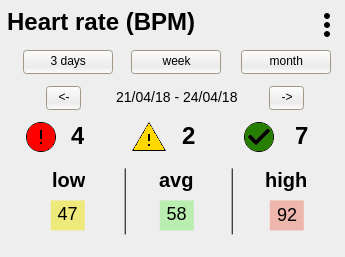
\includegraphics[width=0.45\textwidth]{chapters/3_design/mockups/heart_small}
            \caption{Small heart rate module}\label{fig:hr_small}
        \end{figure}
        \begin{figure}[!htb]
            \centering
            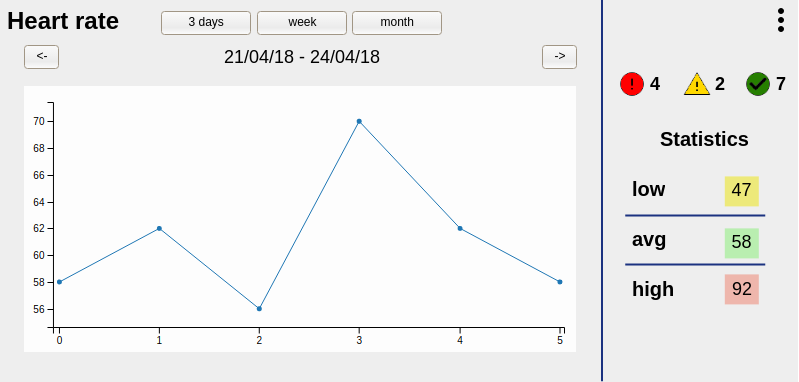
\includegraphics[width=0.75\textwidth]{chapters/3_design/mockups/heart_large}
            \caption{Large heart rate module}\label{fig:hr_large}
        \end{figure}

        The small summarizing module (figure \ref{fig:hr_small}) tries to indicate how the last three, seven, or 30 days went. Three buttons are present to choose the time period. Navigating the time period is done by pressing the arrow buttons. Based on the set thresholds, a count is generated of the measurements: good values lay between the recommended values, warning values lay between the danger and recommended values, and dangerous values have crossed the danger threshold. These are color coded as green, yellow, and red respectively. Below the count, the lowest, average, and highest values for the selected time period are found. These values are again color coded to situate them in the threshold zones. A settings button shows a menu wherein the user can change the thresholds for the current patient. Also, the options to remove or enlarge the module are found here.

        A larger module (figure \ref{fig:hr_large}) provides more detail. The left hand side features a line chart which plots the heart rate measurements over time. Areas on the chart are highlighted green, yellow, or red to indicate the thresholds. Just as the small module, time periods can be selected. To the right of the chart area, the same count and summarizing values are found as in the small module. A simple list of the values was avoided since all the information is present in the graph, although such a list can be added in the future.

        \subsubsection{Blood pressure}
        
        \begin{figure}[!htb]
            \centering
            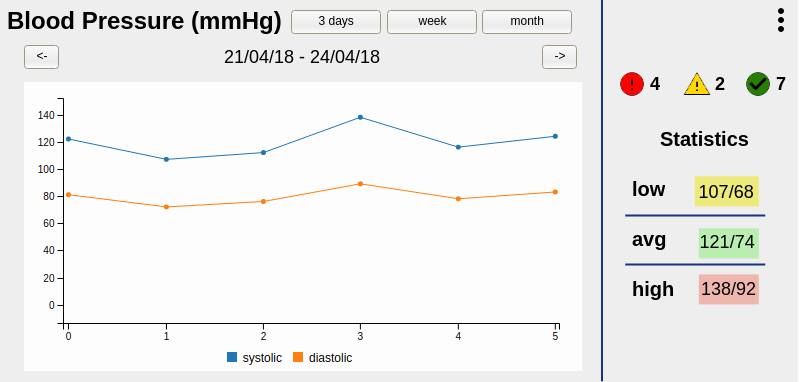
\includegraphics[width=0.75\textwidth]{chapters/3_design/mockups/bp_large}
            \caption{Large blood pressure module}\label{fig:bp_large}
        \end{figure}

        The functionality and design of both the small and large modules are the same compared to the heart rate module. The only difference is that the chart of the large module (figure \ref{fig:bp_large}) displays two lines: one for the systolic blood pressure (BP) and one for the diastolic blood pressure. The threshold zones are also different. Warnings are shown if either the systolic BP is too high or if the diastolic BP is too low. Since both systolic and diastolic BP change in the same direction, this method should suffice. For example, in a hypertensive state both the systolic and diastolic are too high, not just one. If both BP values are between the systolic and diastolic warning zones, the value is flagged as okay.

        \subsubsection{Blood sugar}

        The blood sugar modules are composed the same as the heart rate modules. An issue surrounding blood sugar is the time it was measured: in a fasted state or not. Blood sugar levels differ according to this state. We assume that all blood sugar measurements are taken in a more or less similar setting. It is possible for one patient to measure blood sugar in a fasted state and another patient after a meal, since individual thresholds can be customized.

        \subsubsection{Weight}

        \begin{figure}[!htb]
            \centering
            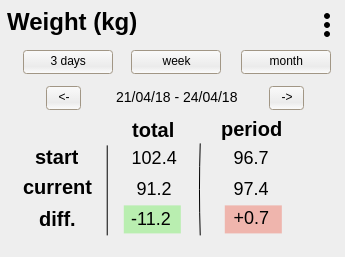
\includegraphics[width=0.45\textwidth]{chapters/3_design/mockups/weight_small}
            \caption{Small weight module}\label{fig:weight_small}
        \end{figure}

        \begin{figure}[!htb]
            \centering
            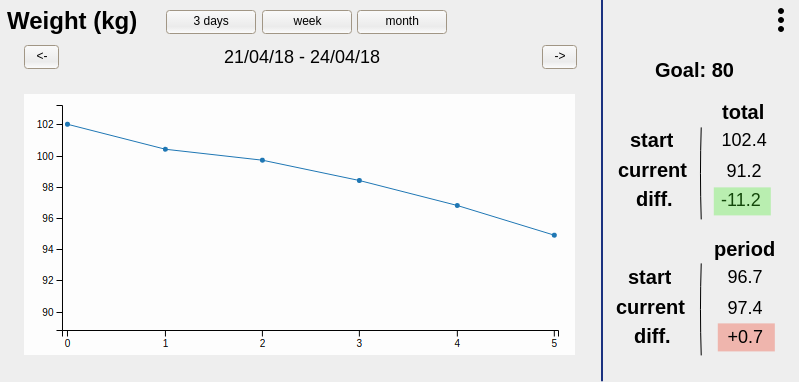
\includegraphics[width=0.75\textwidth]{chapters/3_design/mockups/weight_large}
            \caption{Large weight module}\label{fig:weight_large}
        \end{figure}

        The weight module shows different statistics. To start, there are no thresholds present, only a goal weight can be set. Progress is visualized based on this value. The small module (figure \ref{fig:weight_small}) shows the starting weight (the first measurement ever registered) and the current weight of a patient today (last registered measurement). The difference of these two values is calculated and marked either green or red. If the person is moving closer towards the goal weight, the color will be green and otherwise red. A second column shows the same information, but for values from the selected time period. This allows the clinician to see, for example, the progress made weekly. Similar values are shown in the larger module (figure \ref{fig:weight_large}). It features the same layout as the previous large modules. The chart does not show any colors since there are no thresholds. Instead, a line is shown which represents the goal weight. Ideally, the measured values close in towards this line over time.

        \subsubsection{Oxygen saturation}

        This module group is also very similar to the heart rate ones. The only small difference is present in the thresholds. Blood oxygen levels are generally very high and only if this value is lower than usual, warnings should be issued. Therefore, there are no thresholds when the blood oxygen level is too high, since higher is better.

        \subsubsection{Medication}

        \begin{figure}[!htb]
            \centering
            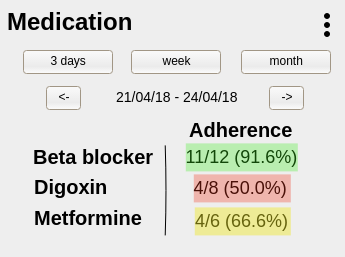
\includegraphics[width=0.45\textwidth]{chapters/3_design/mockups/med_small}
            \caption{Small medication module}\label{fig:med_small}
        \end{figure}

        \begin{figure}[!htb]
            \centering
            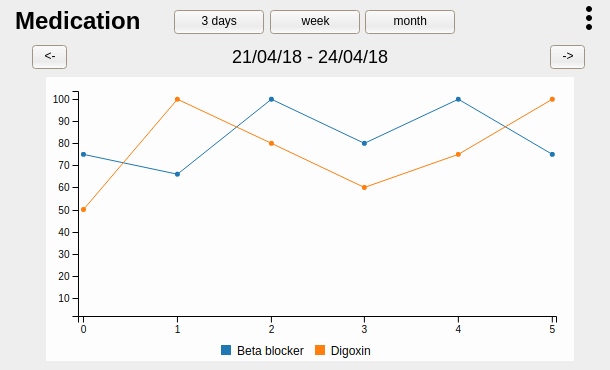
\includegraphics[width=0.75\textwidth]{chapters/3_design/mockups/med_large}
            \caption{Large medication module}\label{fig:med_large}
        \end{figure}

        Medication intake is tracked in a very different manner compared to the previous parameters. It is possible that a patient needs to take in multiple medicines in changing amounts over time. The small module (figure \ref{fig:med_small}) shows all the medicines the patient had to take for the selected time period. Precisely, the actual amount the patient took in, the prescribed amount, and the ratio of these two values. Depending on the thresholds, the background will be color coded red, yellow, or green. These thresholds indicate the minimum ratios the patient must abide by.

        The chart in the large module (figure \ref{fig:med_large}) shows a line for each medicine the patient has to take in. The y-values are the ratios previously discussed and the threshold regions are colored on the chart. The aggregated values from the small module are not shown as the intake trend is visualized on the chart, making the average intake irrelevant. A legend indicates which line represents which medicine. Hovering over a data point indicates this as well.